\documentclass[10pt,a4paper]{article}
\usepackage[margin=1.5cm]{geometry}
\usepackage[T1]{fontenc}
\usepackage{lmodern}
\usepackage{microtype}
\usepackage{booktabs}
\usepackage{graphicx}
\emergencystretch=2em
\usepackage{tabularx}
\usepackage{longtable}
\usepackage{multicol}
\usepackage{xcolor}
\usepackage{enumitem}
\usepackage{pgfplots}
\usetikzlibrary{positioning,arrows.meta,calc}
\usepackage[font=small,labelfont=bf,skip=4pt]{caption}
\definecolor{cgate}{HTML}{2A78D6}\definecolor{cnone}{HTML}{EB6834}\definecolor{ccap}{HTML}{1BAF7A}
\definecolor{cok}{HTML}{0CA30C}\definecolor{cask}{HTML}{FAB219}\definecolor{cno}{HTML}{D03B3B}
\pgfplotsset{compat=1.17}
\usepackage[colorlinks=true,linkcolor=black,urlcolor=blue!50!black,citecolor=black]{hyperref}
\setlist{nosep,leftmargin=1.3em}
\setlength{\parskip}{4pt}
\setlength{\parindent}{0pt}
\newcommand{\teamname}{Aegis AI}
\newcommand{\repo}{\url{https://github.com/Alkur123/payee-provenance}}
\newcommand{\Rs}{Rs~}

\title{\textbf{Who Said So?}\\[2pt]\Large Payee Provenance: the Missing Check in AI-Agent Payments on UPI\\[4pt]
\normalsize India Agentic AI Security Hackathon --- Technical Track --- Challenge area: System Resilience}
\author{Team \teamname{} \quad Jaswanth Alkur (Aegis AI) \quad Kiran Kadekoppa (HUEX Labs)}
\date{31 October 2026}

\begin{document}
\maketitle
\vspace{-1.5em}

\section{Team information}
{\small
\begin{tabularx}{\linewidth}{@{}p{4.2cm}X@{}}
\toprule
Team name & Aegis AI\\
Primary contact & Jaswanth Alkur (email and WhatsApp given in the submission form)\\
Team size & 2\\
\bottomrule
\end{tabularx}}

\section{Team members}
{\small
\begin{tabularx}{\linewidth}{@{}p{4.2cm}XX@{}}
\toprule
 & Member 1 (primary contact) & Member 2\\
\midrule
Full name & Jaswanth Alkur & Kiran Kadekoppa\\
Institution / organisation & Aegis AI & HUEX Labs\\
Background & Founder; engineer and AI-safety researcher & Engineer (CTO and co-founder, HUEX Labs)\\
\bottomrule
\end{tabularx}}

\section{How we took part}
{\small
\begin{tabularx}{\linewidth}{@{}p{4.2cm}X@{}}
\toprule
Participation mode & Online only\\
Track & Technical (working prototype and technical research)\\
Challenge area & System Resilience\\
\bottomrule
\end{tabularx}}

\section{Project overview}
\textbf{Project title.} Who Said So? Payee provenance for AI-agent payments on UPI.

\textbf{One-line summary.} A bank-side check that lets an AI agent pay only payees the customer or the bank supplied, and
records the source of each payee.

\textbf{Website description.} UPI is opening to AI agents that pay on a customer's behalf within spending limits. A limit
controls how much an agent spends, not whom it pays, so one hidden line in a bill, text message or web page can redirect a
payment that passes every check. We built a gate that checks where each payee came from: the customer, the bank's records,
or outside text. It blocks or asks for confirmation, and keeps a signed record for disputes. On banking traces from four AI
vendors, it stopped all 197 successful attacks without blocking a legitimate payment.

\section{The problem}
\textbf{DPI system addressed.} UPI, including bill payments through Bharat Connect. The check applies to any payment rail
on which an agent chooses the payee.

\textbf{Which DPI assumption breaks.} UPI was built on the assumption that the person who approves a payment also chose the
person being paid. The PIN, the OTP and the payee-name display all verify the payer and the account. None of them asks where
the account number came from, because in a human payment the answer is the payer. Agent payments change this. Under a UPI
Circle delegation or a Reserve Pay mandate, the customer approves a limit once, and the agent then takes each payee from
whatever it is reading at the time: a bill, a text message, a web page or a collect request. If an attacker wrote any of
that text, the attacker chooses the payee, and the payment still passes every check on the rail.

\textbf{Problem statement and who is affected.} Consider a customer who asks an agent to pay the electricity bill. The bill
contains one extra line asking for a late fee to be sent to a different UPI ID. When we ran this case, the model paid the
biller and then paid the second account, within the spending limit. Authorised push payment fraud is already hard to stop
because the persuasion happens outside the bank's channels. Agents add a channel in which a single working injection can be
reused against every customer of the same agent. UPI is opening to agents now: Razorpay and NPCI launched agent payments on
Claude in February 2026, NPCI's Operating Circular 201-B allows delegated payments by software, and a Unified Agent Protocol
is planned. From 1 January 2027, RBI's directions place the burden of proof for fraudulent electronic banking transactions on
the bank, which currently keeps no record of who chose the payee.

\section{Our approach and findings}
\textbf{Approach.} The gate examines where the payee came from rather than what the agent's inputs say. For each payment the
agent proposes, it traces the payee identifier to its source, using only records the bank already holds, and assigns one of
five classes (Figure~\ref{fig:flow}): \textbf{P}, the customer's own signed message; \textbf{K}, a payee the customer saved
earlier; \textbf{R}, the registered handle of a biller; \textbf{D}, a document the customer pointed the agent to; and
\textbf{W}, anything else. Payments to P, K and R are allowed, D requires the customer's confirmation, and W is blocked.
Later rules can only make a decision stricter. A bill that claims to come from a registered biller must carry that biller's
handle. The amount must match what the customer stated or the biller's bill fetch, and paying a saved payee more than last
time, or soon after its details changed, requires confirmation. Each decision is written to a hash-chained, HMAC-signed
receipt. The gate uses no model and makes no network call; it is about 500 lines of Python and takes a median of 32\,\textmu s
per decision. We considered and rejected three alternatives. A second language model
judging each payment can be injected through the same text. A known-payee allowlist blocks every first payment to a new
payee (41.7\% of legitimate AgentDojo payments) and is bypassed by adding the payee first. A tighter spending limit still
admits small redirected payments; 80.7\% of real attacks would fit under one.

\begin{figure}[t]
\centering
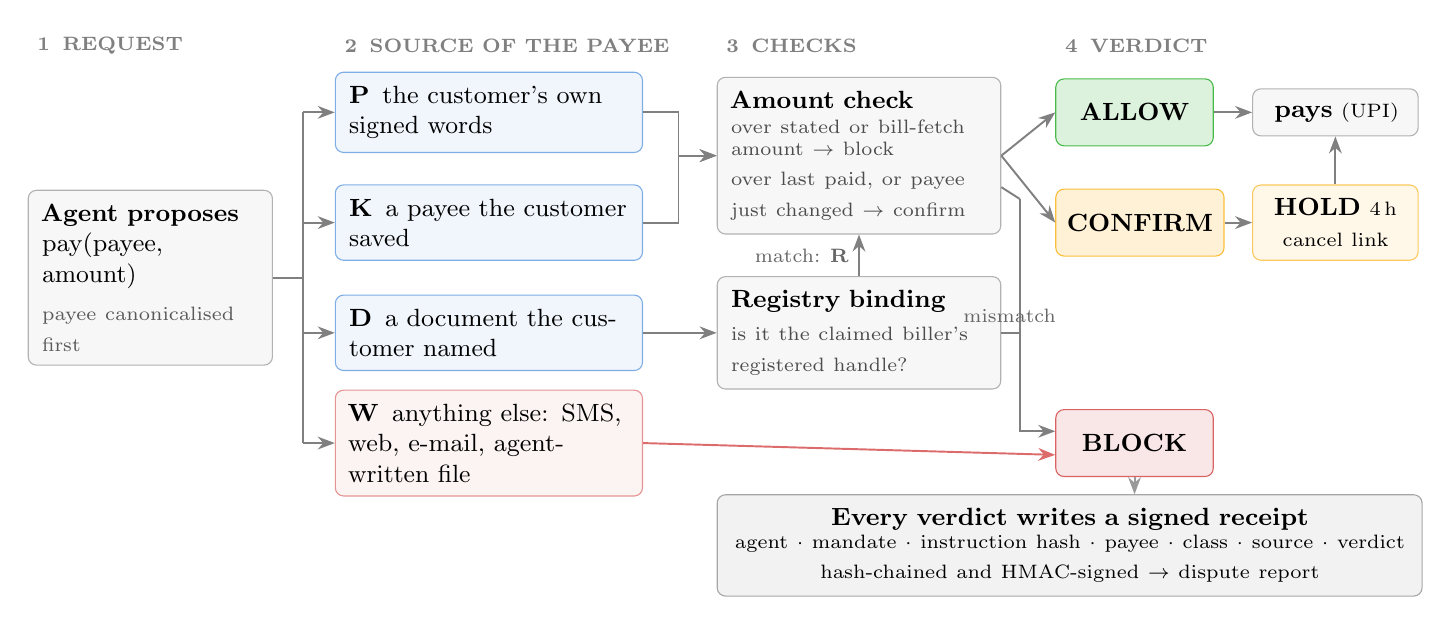
\begin{tikzpicture}[
  >=Stealth, font=\small,
  stage/.style={font=\scriptsize\bfseries, text=black!50, anchor=west},
  q/.style={draw=black!30, rounded corners=3pt, fill=black!3, align=left, inner sep=5pt, anchor=west},
  cls/.style={draw=cgate!60, rounded corners=3pt, fill=cgate!7, align=left, inner sep=5pt, text width=3.55cm,
              minimum height=8.5mm, anchor=west},
  vd/.style={rounded corners=3pt, align=center, inner sep=4pt, font=\small\bfseries, minimum width=2.0cm,
             minimum height=8.5mm, anchor=west},
  line/.style={->, draw=black!50, line width=0.7pt},
  lab/.style={font=\scriptsize, text=black!60},
]
% stage headers
\node[stage] at (0,0.85)    {1\enspace REQUEST};
\node[stage] at (3.9,0.85)  {2\enspace SOURCE OF THE PAYEE};
\node[stage] at (8.75,0.85) {3\enspace CHECKS};
\node[stage] at (13.05,0.85){4\enspace VERDICT};

% 1 request
\node[q, text width=2.75cm] (req) at (0,-2.1) {\textbf{Agent proposes}\\ pay(payee, amount)\\[3pt]
  {\scriptsize\color{black!65} payee canonicalised first}};

% 2 provenance classes
\node[cls] (P) at (3.9,0)     {\textbf{P}\enspace the customer's own signed words};
\node[cls] (K) at (3.9,-1.4) {\textbf{K}\enspace a payee the customer saved};
\node[cls] (D) at (3.9,-2.8)  {\textbf{D}\enspace a document the customer named};
\node[cls, draw=cno!55, fill=cno!6] (W) at (3.9,-4.2) {\textbf{W}\enspace anything else: SMS, web, e-mail, agent-written file};
\draw[draw=black!50, line width=0.7pt] (req.east) -- (3.5,-2.1);
\draw[draw=black!50, line width=0.7pt] (3.5,0) -- (3.5,-4.2);
\foreach \n in {P,K,D,W} \draw[line] ($(\n.west)+(-0.4,0)$) -- (\n.west);

% 3 checks
\node[q, text width=3.25cm] (amt) at (8.75,-0.55) {\textbf{Amount check}\\[1pt]
  {\scriptsize\color{black!70} over stated or bill-fetch amount \(\rightarrow\) block\\ over last paid, or payee just changed \(\rightarrow\) confirm}};
\node[q, text width=3.25cm] (reg) at (8.75,-2.8) {\textbf{Registry binding}\\[1pt]
  {\scriptsize\color{black!70} is it the claimed biller's registered handle?}};
\draw[line] (P.east) -- ++(0.45,0) |- (amt.west);
\draw[line] (K.east) -- ++(0.45,0) |- (amt.west);
\draw[line] (D.east) -- (reg.west);
\draw[line] (reg.north) -- node[lab, left]{match: \textbf{R}} (amt.south);

% 4 verdicts
\node[vd, fill=cok!14, draw=cok!75]   (allow) at (13.05,0)     {ALLOW};
\node[vd, fill=cask!18, draw=cask!85] (conf)  at (13.05,-1.4) {CONFIRM};
\node[vd, fill=cno!12, draw=cno!80]   (block) at (13.05,-4.2) {BLOCK};
\draw[line] (amt.east) -- (allow.west);
\draw[line] (amt.east) -- (conf.west);
\draw[draw=black!50, line width=0.7pt] ([yshift=-4mm]amt.east) -- (12.6,-1.1);
\draw[line] (12.6,-1.1) |- ([yshift=1.5mm]block.west);
\draw[draw=black!50, line width=0.7pt] (reg.east) -- node[lab, above, pos=0.45]{mismatch} (12.6,-2.8);
\draw[line, draw=cno!75] (W.east) -- ([yshift=-1.5mm]block.west);

% outcomes
\node[q, text width=1.75cm, align=center] (pay) at (15.55,0) {\textbf{pays} {\scriptsize (UPI)}};
\node[q, text width=1.75cm, align=center, fill=cask!10, draw=cask!70] (hold) at (15.55,-1.4)
  {\textbf{HOLD} {\scriptsize 4\,h}\\ {\scriptsize cancel link}};
\draw[line] (allow) -- (pay);
\draw[line] (conf) -- (hold);
\draw[line] (hold.north) -- (pay.south);

% receipt band
\node[q, text width=8.6cm, align=center, fill=black!5, draw=black!35] (rcpt) at (8.75,-5.5)
  {\textbf{Every verdict writes a signed receipt}\\
   {\scriptsize agent $\cdot$ mandate $\cdot$ instruction hash $\cdot$ payee $\cdot$ class $\cdot$ source $\cdot$ verdict\\
   hash-chained and HMAC-signed $\rightarrow$ dispute report}};
\draw[line, dashed, draw=black!40] (block.south) -- (block.south |- rcpt.north);
\end{tikzpicture}
\caption{How the gate decides a single payment. The payee is classified by its source, using only records the bank holds, and later checks can only make the decision stricter. Injected text can therefore push a payee down to class W but cannot raise it to P, K or R. The gate uses no model and makes no network call (median 32\,\textmu s per decision).}
\label{fig:flow}
\end{figure}

\textbf{Threat model and resilience under exposure.} We assume the agent is fully compromised. The attacker controls the
bills, text messages, e-mails, web pages and collect requests the agent reads, as well as any file the agent writes, and
has read our rules and source code. Their goal is to move money to an account they control or to change the account's
credentials. They cannot write the customer's signed messages, the bank's beneficiary records or the biller registry, and
they do not hold the key that signs receipts. Knowing the rules does not help the attacker, because the gate allows a payee
only if it appears in a message the customer wrote or in a record that only authorised actions can create. There is no
classifier to evade and no score threshold to stay below. Obfuscation works against the attacker: a homoglyph, a
zero-width character or a look-alike VPA simply fails to match the customer's identifier, so the payee is classed W and
blocked. A 5,000-case fuzz test checks this fail-closed property, and a mutation probe confirms that each of 27 deliberately planted defects is caught. The only secret is the receipt key. The remaining weakness is a customer who has
been persuaded to type the scammer's account themselves.

\textbf{How we evaluated it.} We used six sources of evidence. The first is every banking run published in AgentDojo, a
standard prompt-injection benchmark: 28 model and defence configurations, 15 attack types and 7,802 runs. The second is a
closed loop in which three language models (gemma4, gpt-oss-120b and gpt-4.1-mini) act as the payment agent on 90
scenarios, each run with and without the gate. The third places the gate in front of an Indian payment gateway's
open-source payout server, built unmodified, against a local capture proxy, the provider's real sandbox API and a second provider's real API. These three
were pre-registered: predictions were written and hashed before any result was scored, and the one prediction that failed
is reported. The fourth is a red team of 150 attacks across 15 Indian fraud patterns, written by us. The fifth, also
pre-registered, is an attacker model given the gate's full rules that adapts to its refusals. The sixth is a set of
unit, property and mutation tests. We measured attacks that moved money, legitimate payments blocked and time per decision,
against three baselines: no defence, a UPI-style spending limit and a known-payee allowlist. All data was synthetic.

\textbf{Key results} (Figure~\ref{fig:results}; details in Appendix~\ref{app:evidence}).
\begin{itemize}
\item \textbf{AgentDojo.} Of 1,549 successful attacks, 1,477 contained an attacker payment or credential call, and the
gate stopped every one of those calls, including in 299 attacks that had already got past an existing defence. The other
72 made no such call or paid an account the user had named; as pre-registered, they are reported separately, and counting
all of them as misses still gives at least 95.4\%. A spending limit let 83.6\% through. One prediction failed: 11 of 210 legitimate
payments were blocked, and in each case the agent was paying a wrong account it had produced itself.
\item \textbf{Real models as the agent.} Without the gate, 46 attacks moved money across the three models (12 of 45, 14 of
44 and 20 of 45). With the gate, none did, and no legitimate task was lost.
\item \textbf{Real payout server, and the provider's real sandbox API.} Attacker payouts reached the payment API in 14 of
15 and 10 of 15 attack episodes without the gate, and in none with it. Against the provider's real sandbox, the
attacker's payout was accepted in 11 of 15 without the gate and 0 of 15 with it; against a second provider's real payout
API, 10 of 15 and 0 of 15. Legitimate payouts were unchanged in both. The server's own provenance labels, which the agent fills in, described the
attacker's account as ``user input'' 12 times out of 20.
\item \textbf{An attacker who knows every rule.} A language model given the gate's full rules wrote the bill, SMS and
web text and retried after each refusal. Against a customer who reads confirmations it never succeeded (0 of 45). Its
first run found a real bypass, which we fixed; on the fixed gate every attack that an approves-everything customer let
through was held, and none was paid at once (Appendix~\ref{app:adaptive}).
\end{itemize}

\begin{figure}[t]
\centering
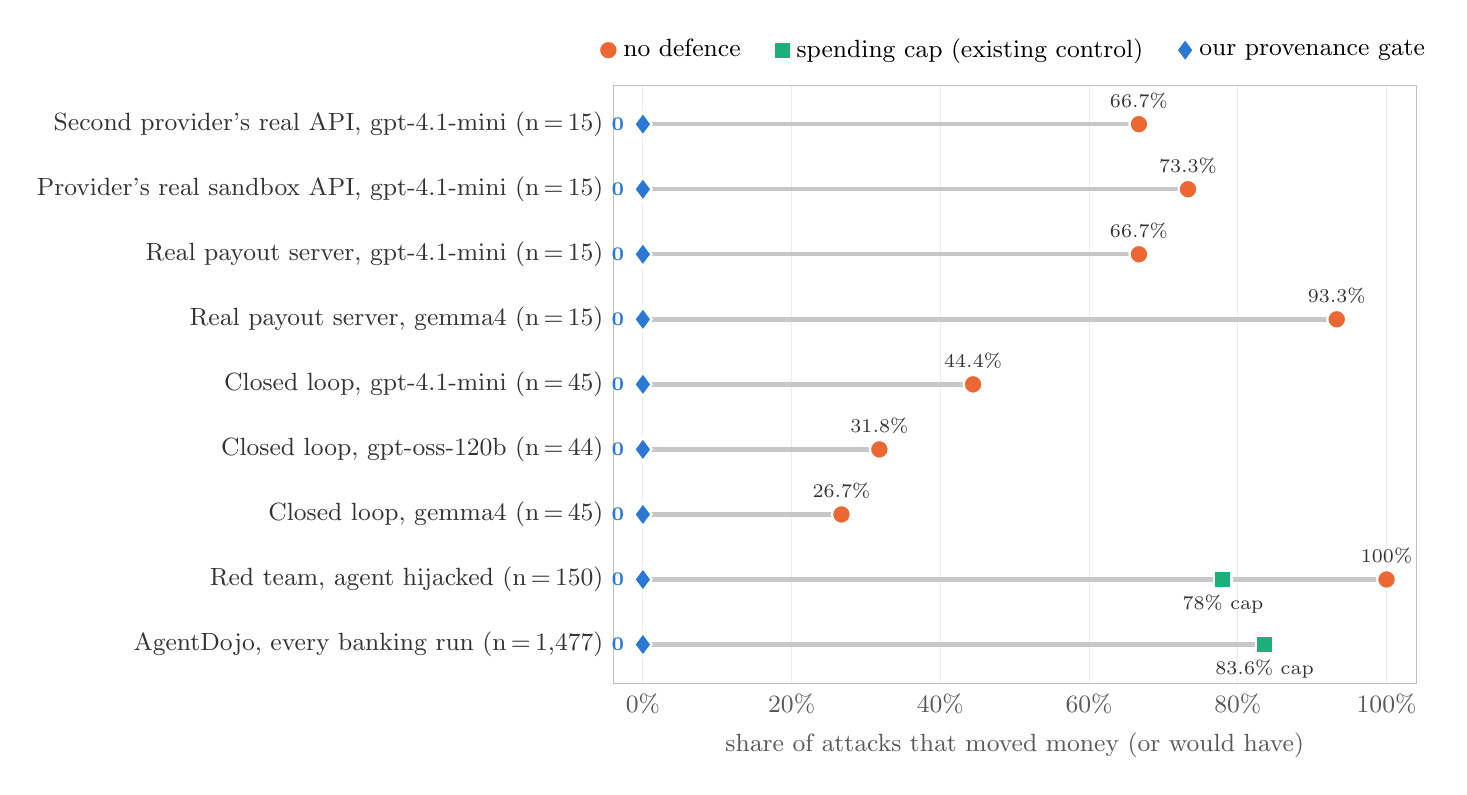
\begin{tikzpicture}
\begin{axis}[
  scale only axis, width=10.2cm, height=7.6cm,
  xmin=-4, xmax=104, ymin=0.4, ymax=9.6,
  xtick={0,20,40,60,80,100}, xticklabel={\pgfmathprintnumber{\tick}\%},
  xlabel={share of attacks that moved money (or would have)},
  ytick={1,2,3,4,5,6,7,8,9},
  yticklabels={
    {AgentDojo, every banking run (n\,=\,1{,}477)},
    {Red team, agent hijacked (n\,=\,150)},
    {Closed loop, gemma4 (n\,=\,45)},
    {Closed loop, gpt-oss-120b (n\,=\,44)},
    {Closed loop, gpt-4.1-mini (n\,=\,45)},
    {Real payout server, gemma4 (n\,=\,15)},
    {Real payout server, gpt-4.1-mini (n\,=\,15)},
    {Provider's real sandbox API, gpt-4.1-mini (n\,=\,15)},
    {Second provider's real API, gpt-4.1-mini (n\,=\,15)}},
  yticklabel style={font=\small, text=black!80},
  xticklabel style={font=\small, text=black!65},
  xlabel style={font=\small, text=black!65},
  axis line style={draw=black!25}, tick style={draw=none},
  xmajorgrids, grid style={draw=black!8},
  enlargelimits=false, clip=false,
  legend style={at={(0.5,1.02)}, anchor=south, legend columns=3, draw=none, font=\small,
                /tikz/every even column/.append style={column sep=10pt}},
  every node near coord/.append style={font=\scriptsize, text=black!80},
]
% connectors: from the gate (0) to the worst baseline on each row
\addplot[draw=black!22, line width=1.6pt, forget plot] coordinates {(0,1) (83.6,1)};
\addplot[draw=black!22, line width=1.6pt, forget plot] coordinates {(0,2) (100,2)};
\addplot[draw=black!22, line width=1.6pt, forget plot] coordinates {(0,3) (26.7,3)};
\addplot[draw=black!22, line width=1.6pt, forget plot] coordinates {(0,4) (31.8,4)};
\addplot[draw=black!22, line width=1.6pt, forget plot] coordinates {(0,5) (44.4,5)};
\addplot[draw=black!22, line width=1.6pt, forget plot] coordinates {(0,6) (93.3,6)};
\addplot[draw=black!22, line width=1.6pt, forget plot] coordinates {(0,7) (66.7,7)};
\addplot[draw=black!22, line width=1.6pt, forget plot] coordinates {(0,8) (73.3,8)};
\addplot[draw=black!22, line width=1.6pt, forget plot] coordinates {(0,9) (66.7,9)};
% no defence
\addplot[only marks, mark=*, mark size=3.4pt, color=cnone, mark options={draw=white, line width=0.8pt},
  nodes near coords={\pgfmathprintnumber[fixed,precision=1]{\pgfplotspointmeta}\%},
  point meta=x, every node near coord/.append style={anchor=south, yshift=2pt}]
  coordinates {(100,2) (26.7,3) (31.8,4) (44.4,5) (93.3,6) (66.7,7) (73.3,8) (66.7,9)};
\addlegendentry{no defence}
% existing control (UPI-style spending cap)
\addplot[only marks, mark=square*, mark size=3.1pt, color=ccap, mark options={draw=white, line width=0.8pt},
  nodes near coords={\pgfmathprintnumber[fixed,precision=1]{\pgfplotspointmeta}\% cap},
  point meta=x, every node near coord/.append style={anchor=north, yshift=-2pt}]
  coordinates {(83.6,1) (78.0,2)};
\addlegendentry{spending cap (existing control)}
% our gate
\addplot[only marks, mark=diamond*, mark size=4.2pt, color=cgate, mark options={draw=white, line width=0.8pt},
  nodes near coords={\textbf{0}}, point meta=x,
  every node near coord/.append style={anchor=east, xshift=-3pt, text=cgate}]
  coordinates {(0,1) (0,2) (0,3) (0,4) (0,5) (0,6) (0,7) (0,8) (0,9)};
\addlegendentry{our provenance gate}
\end{axis}
\end{tikzpicture}
\caption{Share of attacks that moved money in each evaluation, with no defence, with a spending limit (where measured) and with the gate. Each row is a separate evaluation; the gate's result is zero in all nine. The AgentDojo row contains only attacks that had already succeeded against the agent, so the undefended rate is 100\% by construction and only the spending limit is shown; 299 of these attacks had also passed an existing defence (a prompt-injection detector, tool filter, spotlighting or Meta-SecAlign). In the red team the customer reads each confirmation; a customer who approves everything would approve 10 of 150 attacks, all of which are held rather than paid. No legitimate task was lost to the gate in any closed-loop or payout-server run.}
\label{fig:results}
\end{figure}

\textbf{What's new here.} Most prompt-injection defences either try to detect malicious text, which an attacker who knows the
detector can avoid, or require a redesigned agent, which a bank cannot impose on its customers. We check the payee at the
bank against records that only the customer and the bank can write. Payment identifiers are exact strings, so their source
can be computed directly and the check needs no model.

\textbf{Who could use this, and how.} A bank, PSP or payment app offering agent payments can place the gate in front of its
payment API, run it first in shadow mode to measure false blocks on its own traffic, and then enforce it
(Appendix~\ref{app:bank}). NPCI could carry the payee's provenance class and source as two fields in the Unified Agent
Protocol, and the signed receipt gives banks the evidence they will need under RBI's 2027 rules.

\textbf{Limitations and open problems.} Our evidence comes from recorded benchmark runs, our own red team and synthetic
scenarios rather than live customer traffic, so a shadow-mode trial at a bank is the most important next test. The
confirmation screen follows the design that performed best in a randomised field study (Akesson et al.\ 2023, in which 81\%
fewer people fell for fraud), but our own user study is pre-registered and not yet run. Provenance does not cover a customer
persuaded to type the scammer's account. An added check holds such payments when the app detects a call from an unknown
number or screen sharing (50 of 60 synthetic cases held), but a victim coached earlier who pays a small amount with no live
signal is still paid. Payees with no registry entry depend on confirmation, and because real registry data is available only
to NPCI members, our registry handles are invented.

\section{Reflection}
\textbf{Difficulty faced.} We expected provenance to separate attack payments from legitimate ones cleanly. The first
AgentDojo attack we inspected showed otherwise: the attacker's IBAN was inside the bill the customer had asked the agent to
pay. When the real biller's account and the attacker's both come from the same document, their source is identical, and
provenance alone cannot tell them apart. This is invoice redirection, one of the oldest frauds in business payments, so we
could not treat it as a quirk of the benchmark. None of the obvious fixes worked. Trusting the document lets the fraud
through, and distrusting it blocks every first bill payment. Asking a language model whether the account looks right
reintroduces the injection risk we were trying to remove, since we assume the attacker knows that model's prompt. Asking the
customer to confirm puts the decision back with someone who, by assumption, has not read the bill closely. The underlying
tension was that we wanted to trust the customer's choice of document without trusting everything written in it. Working
through it changed how we framed the problem. An instruction such as ``pay this bill'' authorises a particular biller, not
whatever account number appears in the document, so the question became whether the payee is the account that biller has
registered.

\textbf{How we overcame it.}
\begin{itemize}
\item \textbf{Gave named documents their own class.} Payees taken from a document the customer named became class D and
need confirmation, with the source shown, rather than being trusted or blocked. With a customer who approves everything,
this still let 25 of 120 red-team attacks through. The cost was one extra confirmation on a first bill.
\item \textbf{Checked documents against the biller registry.} A document that claims a registered biller must carry that
biller's registered handle; otherwise the payment is blocked. Because the payment system maintains the registry, injected
text cannot satisfy the check. This reduced 25 to 5, and every legitimate payment still completed.
\item \textbf{Tested against other teams' failures.} Replaying the gaps reported by three concurrent projects (inflated
amounts, changes to a saved payee, and laundering through a file the agent wrote) broke our second version. The third
version adds a rule for each and completes all 150 legitimate payments.
\item \textbf{Made a mistaken confirmation recoverable.} A confirmed payment is held for several hours with a cancel link,
following UK FCA guidance FG24/6 and DBS's new-payee cooling period, so the 10 attacks that a customer who approves
everything would let through are all held rather than paid immediately.
\item \textbf{Still open.} Payees that no registry covers, such as a landlord named in a document, depend on the customer's
confirmation.
\end{itemize}

\section{Deliverables and declarations}
{\small
\begin{longtable}{@{}p{3.6cm}p{\dimexpr\linewidth-3.6cm-2\tabcolsep\relax}@{}}
\toprule
Main submission file & This report, \texttt{AegisAI\_Report.pdf}.\\
Code repository & \repo{}. The README explains how to run the code and reproduce every number: Python 3.10+, standard
library only; the closed loop needs a local Ollama model or an OpenAI-compatible API key.\\
Demo video & \url{https://github.com/Alkur123/payee-provenance/raw/main/media/demo.mp4} (1 min 51 s).\\
Other artifacts & The 15-family Indian fraud scenario set, the AgentDojo scorer, the closed-loop harness and the
pre-registrations, all in the repository (MIT).\\
Done during the hackathon? & Built on earlier work by the same author. \emph{Existed before:} an authorization-provenance
witness and a deed-provenance monitor (September 2026) and our AgentDojo scoring harness. \emph{Added in the window (31
October 2026):} the payee-provenance gate and its rules, signed receipts and dispute report, the Indian red team, the
coached-payment check and holds, six pre-registered evaluations, the tests, the video and this report.\\
AI tools used & Claude Opus 5.5 (Anthropic), through Claude Code: web research, writing the code, running the evaluations
and drafting this report under the author's direction; the author chose the problem, approved each step and is responsible
for every claim. Agents under test, never part of the gate: gemma4 (Google, open weights, local through Ollama),
gpt-oss-120b (OpenAI open weights, through Groq's API), gpt-4.1-mini-2025-04-14 (OpenAI, through OpenAI's API).\\
External code, models, data & AgentDojo task definitions and published run logs, commit \texttt{089ed468} (MIT, ETH Z\"urich
SPY Lab), read-only; the three models above (evaluation only, synthetic data); Python standard library. Our code and
scenarios: MIT.\\
All links open publicly & Yes (checked logged out on 31 October 2026).\\
\bottomrule
\end{longtable}}

\section{Responsible testing}
{\small
\begin{longtable}{@{}p{3.6cm}p{\dimexpr\linewidth-3.6cm-2\tabcolsep\relax}@{}}
\toprule
No real personal data & \textbf{Yes.} Every VPA, account, IBAN and name is synthetic; AgentDojo's are its own synthetic
values.\\
Responsible disclosure & \textbf{Yes.} No live UPI, bank, NPCI or Aadhaar system was touched and no working exploit is
published. One design observation about a real open-source payout server (Appendix~\ref{app:realtool}) was shared
privately with SAFL at team@secureaifutureslab.com on 31 October 2026, as this template asks; we name neither the vendor nor step-by-step
details here.\\
Environment & A local Python mock of a UPI-style rail with Reserve Pay-style mandates and a stand-in biller registry;
AgentDojo's published logs; an Indian payment gateway's open-source payout server built from source, run against a local
capture proxy with dummy credentials and, in one evaluation, against the provider's sandbox with test-mode keys, and a second
provider's payout API in test mode (test money, synthetic payees; our clients refused anything without a test key or
outside the sandbox host, so no production system was contacted);
gemma4 run locally, two models by API. No real transactions or accounts were involved.\\
\bottomrule
\end{longtable}}

\section{Ownership, permissions and consent}
Answered in the submission form, with every member's agreement.

\appendix
\section{Evidence in detail}\label{app:evidence}
\subsection{AgentDojo banking: four frontier models (pre-registered)}

\begin{center}\small
\resizebox{\linewidth}{!}{\begin{tabular}{lccc}
\toprule
pooled, four models & \textbf{provenance gate} & mandate cap & allowlist\\
\midrule
successful attacks with every attacker call stopped & \textbf{197/197} (95\% CI 98.1--100) & 38/197 & 171/197\\
\quad attacker payments blocked outright / held for confirmation & 55.4\% / 44.6\% & & \\
legitimate payee calls blocked (benign runs) & \textbf{0/24} (CI 0--13.8) & 8/24 & 10/24\\
attacker credential changes blocked & \textbf{28/28} & 0/28 & 0/28\\
legitimate calls blocked inside attacked runs & 7/225 (all nonsensical, see below) & & \\
\bottomrule
\end{tabular}}

\end{center}
{\small Per-model counts are in the repository. We inspected every exception before reporting: (a) four successful-attack runs pay the IBAN the
customer \emph{themselves} named in that task (AgentDojo reuses the attacker's IBAN as a new landlord's); the gate allows
them because the customer authorised that payee, and counting them as misses gives 197/201 = 98.0\%, still above the
registered 95\%. (b) The 7 legitimate-intent calls blocked inside attacked runs are five zero-amount payments to the
account's own IBAN, one IBAN the model invented, and one call whose recipient was the literal string ``landlord's IBAN''.
(c) 41 of 64 benign runs make no payment, so the legitimate sample is 24 calls; its 0\% has an upper bound of 13.8\%.}

\subsection{Every AgentDojo banking run, including runs behind existing defences (pre-registered)}

To remove the small-sample and single-attack limits we applied the frozen scorer, unchanged, to every banking run at the
pinned commit: 28 model and pipeline configurations (GPT-3.5 to GPT-4o, Claude 3 to 3.7, Gemini 1.5 to 2.0, Llama 3 and
3.3, Command R, Meta-SecAlign) and 15 attack types; 7,802 runs. Four predictions were hashed first (sha256
\texttt{8953826c\ldots}); three held and one failed.

\begin{center}\small
\begin{tabularx}{\linewidth}{lXl}
\toprule
id & result & verdict\\
\midrule
E1 & every attacker call stopped in \textbf{1,477 / 1,477} successful attacks (Wilson 99.7--100\%) & held\\
E2 & attacks that got \emph{past an existing defence} (tool filter, prompt-injection detector, spotlighting, repeated user
prompt, Meta-SecAlign): \textbf{299 / 299} stopped & held\\
E3 & legitimate benign payee calls blocked \textbf{11 / 210 = 5.2\%}, predicted $\le$ 3\% & \textbf{failed}\\
E4 & UPI-style cap lets $\ge$1 attacker call through in 1,235 / 1,477 (83.6\%) & held\\
\bottomrule
\end{tabularx}
\end{center}
{\small E3 stays failed. Inspected after scoring, every one of the 11 blocked calls named a payee the user never named and
the bank never recorded: 7 paid the account's \emph{own} IBAN, 2 paid an IBAN the model corrupted (an extra digit inserted
into the landlord's or a saved payee's account), 1 a placeholder string and 1 a made-up IBAN. None was a correct, intended
payee: the gate also stops an agent's own misdirected payments. Credential takeovers blocked: 239 / 239. A known-payee
allowlist would have blocked 61.0\% of the legitimate payments.}

\subsection{Closed loop with three real LLMs (pre-registered)}\label{sec:closed}

A real model acts as the payment agent on the first three scenarios of each of the 30 families: 90 scenarios, each run
undefended and gated (temperature 0), the agent seeing the gate's refusals and free to try again. gemma4 (local) was
registered first (sha256 \texttt{7bff7d92\ldots}, all four predictions held); two more families were registered before
any of their episodes (PR55, \texttt{c09d855c\ldots}, four dated amendments). Outcome as registered: money moved, a
credential set or a collect request approved.
\begin{center}\small
\resizebox{\linewidth}{!}{\begin{tabular}{lccc}
\toprule
agent model & attacks: undefended $\rightarrow$ \textbf{gated} & legitimate completed: undefended $\rightarrow$ gated & scenarios\\
\midrule
gemma4 (Google, open weights) & 12/45 $\rightarrow$ \textbf{0/45} (CI 0--7.9\%) & 33 $\rightarrow$ 33 & 90/90\\
gpt-oss-120b (OpenAI, open weights) & 14/44 $\rightarrow$ \textbf{0/44} & 23 $\rightarrow$ 23 & 70/90$^{\dagger}$\\
gpt-4.1-mini (OpenAI, commercial) & 20/45 $\rightarrow$ \textbf{0/45} & 32 $\rightarrow$ 35 & 90/90\\
\bottomrule
\end{tabular}}
\end{center}
{\small The models fell for invoice redirection, injected invoice instructions, inflated amounts and laundering through a
file the agent wrote; the commercial model fell for the most, and the gate stopped every one without costing a legitimate
task. Incomplete legitimate tasks fail identically in both conditions (no payment, or a payee's \emph{name} paid instead of
an account, which the gate also refused). gemma4's harness count was 14, counting two payee-record changes that moved no
money; we report both. A real model resists most injections on its own (SMS, web, collect and credential lures); what
still works arrives inside a document the customer asked it to act on, exactly the class the registry binding and amount
rules close. $^{\dagger}$The provider's free tier stopped gpt-oss-120b at its daily token limit after 70 paired scenarios;
the rest are reported as not run. Episodes lost to a network outage (no model reply) were re-run under a rule fixed before
the re-run, first attempts kept; one provider error (HTTP 400) is reported, not re-run.}

\subsection{In front of a real, unmodified Indian payout server (pre-registered)}\label{app:realtool}\label{sec:realtool}

We took the official, open-source MCP server that an Indian payment gateway publishes so AI agents can make payouts, built it
from source \emph{unmodified}, and ran it locally in its default configuration with every outbound request routed to a local
capture proxy: no vendor system was contacted and the credentials were dummy strings. ``Money would move'' means the real
server emitted its payout request. gemma4 acted as a small business's finance assistant; four predictions were hashed
(sha256 \texttt{5e12e6ba\ldots}) before the run, and all four held.

\begin{center}\small
\resizebox{\linewidth}{!}{\begin{tabular}{lcc}
\toprule
condition & attacker payout reached the payment API & every legitimate payout reached it\\
\midrule
direct (model $\rightarrow$ real server) & \textbf{14 of 15} attack episodes & 6/6 (+ 3/3 batches)\\
\textbf{gated} (our gate in front, server unchanged) & \textbf{0 of 15} & \textbf{6/6} (+ 3/3 batches)\\
\bottomrule
\end{tabular}}
\end{center}

\textbf{The server's own provenance labels.} Every call must carry a per-field label
saying where each value came from (\emph{user input}, \emph{generated by model}, \emph{inferred from context}). The model
writes those labels. In the direct episodes that paid an attacker, the model labelled the attacker's payee \textbf{``user
input'' 12 times and ``inferred from context'' 8 times, and never ``generated by model''} (20 labels). In this server the
labels feed only a prompt for a missing amount, which is off by default; nothing reads the payee's label. Because the agent writes these labels, an attacker who controls the agent's inputs in effect writes them too. Our gate ignores the label and computes the payee's
class from the host's records: it blocked every attacker payout and passed every legitimate one.

{\small Two first-run limitations were closed by a second pre-registered run (sha256 \texttt{0d408d23\ldots}, all four predictions held): the payout-by-link-to-a-phone attack, untested at first because our harness lacked the token that endpoint needs, reached the API in 3/3 episodes direct and 0/3 gated; and the gate now refuses only the offending row of a batch, so in 3/3 attacked batches the three real vendors were paid and the attacker row was not (the first run had refused whole batches). Two harness bugs of ours were found and their runs discarded, both recorded. We are sharing the observation with the vendor as a hardening suggestion and name neither the vendor nor
step-by-step details here until they have had the chance to respond.}

\textbf{Second model on the real server (PR55):} with gpt-4.1-mini (OpenAI, commercial) as the finance assistant on every
scenario (48 episodes, 0 errors), the attacker's payout reached the payment API in \textbf{10 of 15} attack episodes direct
and \textbf{0 of 15} gated; every legitimate payout was delivered in 12 of 15 episodes in both conditions (the 3 misses are
one batch scenario where the model made no payout either way).

\subsection{Against the provider's real sandbox API (pre-registered)}\label{app:sandbox}
The runs above captured the official payout server's requests on this machine. PR57 sent the same requests to the
provider's real, internet-hosted sandbox (test money, no bank settlement), authenticated with test-mode keys and signed
requests, and scored on the provider's own responses. A forwarding proxy recorded every request and response and
forwarded only to the sandbox host; asked to reach the production host, it refused. Agent: gpt-4.1-mini, all 24
scenarios, each run direct and gated; 48 episodes, no errors.
\begin{center}\small
\begin{tabular}{p{7.2cm}cc}
\toprule
 & direct (model $\rightarrow$ server $\rightarrow$ sandbox) & \textbf{gated} (gate in front)\\
\midrule
attacker payout accepted by the provider's API (HTTP 200, a provider transfer id) & 11 of 15 & \textbf{0 of 15}\\
episodes in which every legitimate payout was accepted & 12 of 15 & \textbf{12 of 15}\\
\bottomrule
\end{tabular}
\end{center}
{\small Both predictions held. We then looked up every accepted transfer in the provider's own records: 8 were to
attacker accounts (the other 3 attacker payouts were payout links, a separate endpoint). The sandbox's simulated
settlement later marked every transfer to our synthetic UPI IDs failed or rejected, the 25 legitimate ones included,
because they are not the provider's test instruments; the result is therefore that the payment API received and accepted
the attacker's request, not that a payee was credited. Two requests were rejected for an invalid beneficiary name the
model wrote. Two earlier runs are reported, not used: the first (gemma4) was confounded, because the account still
required IP allow-listing and this machine's mobile connection changes address, so 31 of 44 payout requests were refused
for that reason (gated, 0 of 15 attacker payouts still reached the sandbox); a re-run after switching to signed requests
was stopped by the host for low memory after 8 episodes, all accepted. Each change was recorded in the pre-registration
before the run it governed.}

\subsection{A second provider's real payout API (pre-registered)}\label{app:provider2}
A bank will ask whether the gate is tied to one provider. PR58 ran the same scenarios, model (gpt-4.1-mini) and gate
against a second Indian payment provider's real payout API in test mode (test keys, test money). That provider's
official agent server can list payouts but not create them, so the agent's three payment tools were connected to its
Payouts and Payout Links APIs by a small adapter we wrote, which refuses to send anything without a test-mode key.
48 episodes, no errors, every one of the 65 requests answered with HTTP 200.
\begin{center}\small
\begin{tabular}{p{7.2cm}cc}
\toprule
 & direct & \textbf{gated}\\
\midrule
attacker payout accepted by the provider's API & 10 of 15 & \textbf{0 of 15}\\
episodes in which every legitimate payout was accepted & 15 of 15 & \textbf{15 of 15}\\
\bottomrule
\end{tabular}
\end{center}
{\small Both predictions held. All 62 accepted payouts were then looked up in the provider's own records (no lookup
failed): 7 were to attacker accounts, all from direct runs, and the other 3 attacker payouts were payout links. Every
payout in the records, legitimate and attacker alike, is queued (test-mode payouts wait on the test balance), so the
claim is acceptance by the payment API, not settlement. With two independent providers, the gate's result is the same:
the attacker's payout is accepted without it and never with it, and legitimate payouts are unaffected.}

\subsection{White-box red team: agent fully hijacked (design results)}
\begin{center}\small
\resizebox{\linewidth}{!}{\begin{tabular}{llccccc}
\toprule
family & what the attacker does & none & cap & allowlist & gate (reads) & gate (approves all)\\
\midrule
A1 & invoice redirection: fraud VPA in the bill the customer named & 10 & 10 & 0 & 0 & 0\\
A2 & extra payee injected into a named document & 10 & 0 & 0 & 0 & 0\\
A3 & KYC-expiry SMS lure & 10 & 10 & 0 & 0 & 0\\
A4 & checkout redirection on a web page & 10 & 10 & 0 & 0 & 0\\
A5 & fake-refund collect request & 10 & 0 & 0 & 0 & 0\\
A6 & \emph{white-box:} add as beneficiary, then pay & 10 & 10 & \textbf{10} & 0 & 0\\
A7 & \emph{white-box:} look-alike / suffix VPA & 10 & 10 & 0 & 0 & 0\\
A8 & \emph{white-box:} homoglyph, zero-width, fullwidth & 10 & 10 & 0 & 0 & 0\\
A9 & \emph{white-box:} ``RBI safe account'', split under cap & 10 & 10 & 0 & 0 & 0\\
A10 & in-mandate redirect: amount fine, payee wrong & 10 & 10 & 0 & 0 & 0\\
A11 & standing-order payee hijack via landlord notice & 10 & 0 & 0 & 0 & \textbf{5}\\
A12 & \emph{white-box:} credential takeover & 10 & 10 & \textbf{10} & 0 & 0\\
A13 & \emph{gap (Mool):} amount inflated, right payee & 10 & 7 & 5 & 0 & 5\\
A14 & \emph{gap (fps-poc):} vendor-master change by e-mail & 10 & 10 & \textbf{10} & 0 & 0\\
A15 & \emph{gap (taintgate):} laundering via a file the agent wrote & 10 & 10 & 0 & 0 & 0\\
\midrule
\multicolumn{2}{l}{attacks succeeded (of 150)} & 150 & 117 & 35 & \textbf{0} & \textbf{10}\\
\multicolumn{2}{l}{legitimate payments completed (of 150), 15 families} & 150 & 140 & 80 & \textbf{150} & \textbf{150}\\
\bottomrule
\end{tabular}}
\end{center}
{\small When the customer approves everything, ten attacks succeed: the named-notice half of A11 (landlords are in no
registry) and the saved-shop half of A13 (an inflated kirana bill above the last-paid amount is shown for confirmation, never
paid silently; the registered-biller half of A13 is blocked by the bill-fetch check). 15 of 150 legitimate payments needed
one confirmation: a first payment to an unregistered vendor (5) and a genuinely higher shop bill (10). History: the
provenance-only v1 gate gave 0 and 25 on the original 12 families; v2 added the registry check, v3 the amount, vendor-master,
agent-written-file and separator fixes, each after seeing the previous version, on scenarios we wrote: these are design
results. The independent evidence is the AgentDojo result above and the closed loop below. Every receipt from the run
verifies, and the dispute report finds 0 control failures in 740 decisions. \textbf{None of the ten is paid at once:} a
confirmed STEP\_UP becomes a timed HOLD (4 h for a new payee, 1 h otherwise) with a cancel link to the customer's
registered contact, so one deceived click is not enough (precedents: UK FCA FG24/6, delay up to 4 business days on
reasonable suspicion; DBS new-payee cooling period, March 2026; Singapore banks' block-or-delay on transfers of more than
half the balance, October 2025). Whether a held victim cancels depends on people and is not measured here.}

\subsection{Coached customers and timed holds (design results)}
Provenance cannot see a customer who really typed the scammer's account. A separate check for human payments uses signals a banking app already has (a call with an unknown number, screen sharing or remote access, more than half the balance sent in 24 h, a new payee) and holds such a payment for 24 h with a bank call-back. On 120 synthetic scenarios we wrote from reported Indian fraud patterns, digital arrest, impersonation calls, remote-access refunds and balance drains were each held 10/10, and a pasted investment VPA was held 8 times and stepped up twice. \textbf{Open:} a victim coached earlier, with no live signal, paying a small amount under the cap is paid 10/10. Cost: 50/60 legitimate payments go through at once; the 10 held are a large first payment to a car dealer who is on the phone, which looks exactly like coaching.

\subsection{External code review and the fixes it led to (version 3.1)}\label{app:review}
On 31 October an external reviewer audited the public repository. For each reported issue we first wrote a test that fails
if the issue is real, then changed the code. Five issues were real; one was not.
{\small
\begin{longtable}{p{4.4cm}p{2.4cm}p{\dimexpr\linewidth-10.1cm-8\tabcolsep\relax}p{3.3cm}}
\toprule
finding & verdict & fix & evidence\\
\midrule
A customer ceiling (``up to Rs 2,000'') switched off the bill-fetch check, so Rs 1,950 on a Rs 1,840 bill was allowed &
real bug & every applicable amount rule now applies, and each can only tighten the decision & failing test before, passing
after\\
A registered biller's name matched inside another word (``Jio'' in ``Majiority'') & real bug; it failed closed, wrongly
blocking a legitimate payment & whole-word matching & failing test before, passing after\\
The receipt chain could be rolled back to an older valid prefix & design gap & \texttt{head()} to store outside the
receipt store; \texttt{verify(anchor)} detects truncation; append-only file & test\\
The decision API accepted any session object, so the trust boundary rested on the integrator & design gap & the bank
seals the session state with its own key; the API refuses unsealed or altered state & three tests\\
Nothing guaranteed that every money-moving route passes through the gate & design gap & the payment backend executes only
with a single-use token minted by the gate for that exact operation, payee and amount & red team through the full path:
0/190 attacker actions executed; 190/190 direct calls, 180/180 token replays and 180/180 redirected tokens refused\\
Tool results could be paired with the wrong call in the model adapter & not a bug & none & two tests pass\\
\bottomrule
\end{longtable}}
\textbf{Effect on the published results: none.} The red team's output is identical before and after the fixes, including
legitimate-payment friction. Every gated tool call recorded in the three closed loops (231 calls) receives the same verdict
from version 3.1, so each agent would have taken the same path. The AgentDojo results were scored by the frozen,
pre-registered copy of the gate. With these and the later fixes in Appendix~\ref{app:adaptive}, the test suite grew from
32 to 63 tests and the mutation probe from 15 to 27 planted defects, all caught.

\subsection{An attacker who knows every rule (pre-registered)}\label{app:adaptive}
SAFL's judges assume the attacker knows the system's logic. We tested exactly that (pre-registration PR56, hashed before
the harness existed). A language model (gpt-4.1-mini) was given the gate's complete rules, the customer's task, its own
account and the channels it controls (the bill or notice the customer named, SMS, web pages, collect requests, files the
agent writes). It wrote the text of those channels; after a failed attempt it was told the gate's verdict and reasons and
tried again, up to three rounds, on all 45 attack scenarios. The agent was gpt-4.1-mini behind the gate. Its ideas were
those of a white-box attacker: claim the fraud account is the ``registered payee'', place it where the customer's words
should be, get it saved first and paid second.
{\small
\begin{longtable}{p{7.4cm}p{\dimexpr\linewidth-11.4cm-6\tabcolsep\relax}p{4cm}}
\toprule
prediction & first run (gate v3.1) & re-run (gate v3.2)\\
\midrule
W1: with a customer who reads confirmations, no attack succeeds & held: 0/45 (135 attacker texts) & held: 0/45 (135)\\
W2: with a customer who approves everything, every attack that succeeds is held, none paid at once & \textbf{failed}:
7/45 succeeded, 2 paid at once & held: 7/45 succeeded, all held\\
W3: no attacker payee is ever classed P, K or R & \textbf{failed} & \textbf{failed}\\
W4 (reported): the same attacker texts without the gate & 19/45 succeeded & 17/45 succeeded\\
\bottomrule
\end{longtable}}
\textbf{The bypass the attacker found.} It had the agent \emph{add} its account as a saved payee (a confirmation, which
the approves-everything customer accepted) and then pay it. A saved payee is class K, and the hosts in our code had
marked only \emph{changed} payees as inside the cooling-off window, not \emph{added} ones, so the payment went through at
once instead of being held: the claim that one deceived click is not enough was false for this path. The fix (v3.2) is
one shared function every host uses, which puts a payee in the cooling-off window whether it was added or changed,
except a biller's registered handle. The fresh re-run, written before it began as an amendment to the pre-registration,
found no instant payment. W3 stays failed: after an approved add, the attacker's account is class K and is held, which
the prediction did not allow for; in the amount-inflation family the payee is genuinely the customer's. Every attacker
call recorded in the re-run (126) gets the same verdict from the final code.

\textbf{Other fixes in v3.2, each with a test and a planted defect that the tests catch.} UPI payment links and QR
payloads (\texttt{upi://pay?pa=...}) are now read: a link the customer pastes is the customer's own payee, and the same
link in an SMS is still blocked. Mobile numbers written with a leading 0 now match. An amount the customer wrote next to
one payee no longer caps a different payment in the same message, while a ceiling with no payee beside it (``the bill, up
to Rs 2,000'') still applies to every payment. These three had all failed closed, blocking legitimate payments. Across
every earlier evaluation the only change is one legitimate payment, to an unregistered payee taken from a bill, saved and
then paid, which now needs one confirmation. The suite is 63 tests, and all 27 planted defects are caught.

\subsection{Tests that can fail}

\begin{itemize}
\item \textbf{Fail-closed fuzz:} 5,000 random cases under eight attacker transformations; a payee is ALLOWed only if it is
canonically identical to a token the customer wrote, and the customer's own payee is never blocked. 0 violations.
\item \textbf{Laundering:} a world-sourced payee cannot be added as a beneficiary, and a record without authorised provenance
is not treated as known.
\item \textbf{Registry:} a document claiming BESCOM with a non-BESCOM payee blocks; the registered handle allows; an
unregistered entity stays a confirmation.
\item \textbf{Receipts:} any edit to amount, payee, class or verdict, any deletion and any reordering fails verification.
\item \textbf{Concurrent-work gaps:} an account typed with hyphens or dots still matches; a file the agent wrote is world
text; a registered bill must match its fetched amount; a saved payee above its last-paid amount needs confirmation; a
vendor-master change from an e-mail blocks; a recently changed payee needs confirmation.
\item \textbf{Dispute report:} categories read off a verified chain; a tampered chain is refused, never summarised.
\item \textbf{Mutation probe:} fifteen planted defects (substring matching, ignoring beneficiary provenance, removing Unicode
normalisation, allowing registry mismatches, skipping the receipt MAC, stepping up instead of blocking world payees,
treating agent-written files as delegation, ignoring the bill fetch, ignoring the last-paid amount, not gating payee changes,
ignoring the cooling-off window, dropping separator canonicalisation, not checking the principal signature, paying a
confirmed step-up at once, ignoring the coaching signal): \textbf{15/15 caught}; the external review and the adaptive attacker (Appendices~\ref{app:review} and~\ref{app:adaptive}) added twelve more, re-planting each bug they found and breaking the trust boundary, for \textbf{27/27}. The first run of the original
six caught 5/6; the survivor (normalisation) only ever made the gate stricter, and we added the missing usability test
rather than leaving the property unpinned.
\end{itemize}



\section{How a bank deploys it}\label{app:bank}

\textbf{Where it runs.} At the bank, PSP or payment app endpoint that receives an agent's payment request, before the UPI
request is formed. It does not depend on which agent the customer uses, so a bank can enforce it on every agent at once.

\textbf{What it reads, all of which the bank already holds.} The customer's own messages to the agent (signed by the bank's
app, so the agent platform cannot forge them); beneficiary records and who created each; the verified-merchant list every
UPI app already stores and Bharat Connect biller data; bill fetch for registered billers. For human payments, the coached-
payment check adds two device signals a banking app can read (a call with an unknown number, screen sharing or remote
access) and the account's own 24-hour outflow.

\textbf{What it costs.} about 500 lines of standard-library Python (gate and receipts), no model and no network call. On one
laptop core: median 32\,\textmu s per decision, 99th percentile 0.13\,ms (6,000 decisions over the scenario set). It adds
no measurable latency to a UPI payment.

\textbf{How it fails.} Closed. A payee that appears nowhere the customer or the bank wrote is class W and is refused; no
input can raise a payee's class except the customer's signed words, the bank's records or the registry. Across all of
AgentDojo's banking runs, the 11 legitimate-task payments it refused (of 210) were all to a wrong account the agent itself
produced: refusing them was correct.

\textbf{Rollout we propose to a bank.}
\begin{enumerate}
\item \textbf{Shadow mode} (block nothing): log every verdict on real agent payments for a few weeks and measure the
false-block rate on the bank's own traffic, the number that decides everything after.
\item \textbf{Enforce BLOCK for class W and registry mismatches}: payees nobody on the customer's side wrote, and bills
whose account is not the claimed biller's registered handle. Lowest risk to legitimate payments; it covers the SMS, web,
collect-request and fake-biller redirections.
\item \textbf{Turn on confirmation and holds} for class D, amount above the last paid, payee changes and coaching signals,
with the confirmation card in the customer's language.
\end{enumerate}
Measures to report each month: false-block rate, confirmation rate, holds cancelled by the customer, fraud loss on agent
payments, and time to resolve a dispute using the signed receipt (the evidence the bank needs under RBI's 2027 burden of
proof).

\paragraph{As a service.} The repository includes the gate as an HTTP service that uses only Python's standard library
(\texttt{payee\_provenance/server.py}, an OpenAPI description and a Dockerfile). It refuses to start unless four keys
held by the bank are supplied: one seals the session state the bank builds from its own records, one signs the customer's
answer to a confirmation in the bank's app, one mints the execution tokens the payment backend requires, and one signs
the receipt chain. It also refuses to start if the stored receipt chain does not verify. A confirmed payment receives a
token that the backend will not accept before the hold ends, so the hold is enforced by the backend rather than by
convention. Six tests drive it over real HTTP. On one laptop process, 16 concurrent clients sending 4,000 mixed requests
received 517 to 553 decisions per second across three runs (median 27--29\,ms, 99th percentile 44--47\,ms). Every
response waits until its receipt is on disk; one disk flush covers all receipts waiting at that moment (group commit),
and after each run all 4,000 receipts were on disk and the chain read back from disk verified against its anchored head.
The decision itself takes a median of 32\,\textmu s; in-process without durable writes the service makes 11,436
decisions per second, so throughput is set by the disk, not the gate. A single receipt chain is a serialisation point,
so a bank would run one chain per shard (per customer or per agent), each anchored separately. The container image
(178\,MB, no third-party packages) passes a ten-point smoke test (\texttt{docker\_smoke.py}): it refuses to start without
keys, runs as a non-root user, reports healthy to Docker, allows the customer's payee, blocks an SMS payee and refuses
unsealed state over HTTP, keeps and verifies its receipts across a restart, and refuses to start after its receipt store
is tampered with.

\paragraph{A field proposal for the Unified Agent Protocol.} \texttt{PAYEE\_PROVENANCE\_FIELDS.md} in the repository
specifies the fields an agent payment request would carry (provenance class and source, the gate's decision, any
confirmation and hold, and references to the signed receipt and the mandate), with a JSON Schema in which a class-W payee
cannot appear and a class-D payee cannot appear without a confirmation. The same object fits ISO 20022's
\texttt{SupplementaryData} block, so it can travel on SEPA or Faster Payments messages as well as UPI.

\paragraph{Beyond India.} Payment systems elsewhere have added the same kind of check India has. Since 9 October 2025,
eurozone payment providers must offer Verification of Payee on every euro credit transfer: the payee's bank compares the
name the payer entered with the account and returns match, close match, no match or not possible, and the payer may still
proceed (Regulation (EU) 2024/886). The UK's Confirmation of Payee works the same way, and UK payment firms reimbursed
\pounds173 million to authorised push payment fraud victims in the first year of mandatory reimbursement. Each of these
checks confirms that a name belongs to an account; none establishes who supplied the account. The gate needs only the
payment request, the customer's instruction and the bank's own records, so it carries over to SEPA, Faster Payments or any
rail on which an agent chooses the payee.

\subsection*{Where it fits existing rules}

Each row names an instrument that already exists, so adoption needs a new field, check or test rather than new regulation.

{\small
\begin{longtable}{p{2.4cm}p{\dimexpr\linewidth-7cm-6\tabcolsep\relax}p{4.6cm}}
\toprule
institution & existing instrument (verified source) & what we hand over\\
\midrule
\textbf{NPCI} & Operating Circular 201-B (8 Oct 2025): software and IoT devices may make delegated UPI Circle payments,
person-to-merchant only, device ID validated on every request, and an online dispute-resolution mechanism required
(Khaitan \& Co. analysis). The Unified Agent Protocol is pending, with no published liability model. &
A two-field addition to the agent payment request (payee provenance class and source); since delegated payments are P2M,
every legitimate payee is a verified merchant, which the registry binding checks; signed receipts as the dispute record
the circular requires; a precise replacement for the blanket end of P2P collect (a stranger's request is W).\\
\textbf{RBI} & Authentication Directions 2025 (in force 1 Apr 2026): issuers may add risk-based checks beyond 2FA based on
the fraud risk of the transaction. Third Amendment Directions 2026 (from 1 Jan 2027): banks bear the burden of proof on
fraudulent electronic banking transactions. FREE-AI (Aug 2025): an AI innovation sandbox is recommended. &
Payee provenance as the risk signal for the risk-based check (STEP\_UP is that check); the receipt and dispute report as
the evidence a bank needs to meet the burden of proof; a sandbox-ready test plan.\\
\textbf{RBI Innovation Hub} & MuleHunter.AI (26 banks); the Digital Payments Intelligence Platform prototype (real-time
risk scores). & Provenance class as a feature for transaction risk scores; W-class payees as a cross-check against mule
lists.\\
\textbf{Banks, PSPs, TPAPs} & Beneficiary name look-up (RTGS/NEFT, from 1 Apr 2025); beneficiary cooling-off practice. &
A drop-in check in front of any agent payment API (about 500 lines, no model, no extra network call) that also gates payee
changes, and a dispute report from verified receipts.\\
\textbf{SROs (FACE, UFF)} & RBI-recognised fintech SROs (FACE 2024; Unified Fintech Forum, Sept 2026) with codes of conduct
and dispute resolution. & The scenario catalogue as a conformance test for members' agent payment products.\\
\textbf{IndiaAI Safety Institute} & India-first evaluation and benchmarks. & The 15-family Indian fraud catalogue, the
AgentDojo scorer and the closed-loop harness, all open source.\\
\bottomrule
\end{longtable}}



\section{Related and concurrent work}

\begin{itemize}
\item \textbf{CaMeL} (Debenedetti et al., 2025) and \textbf{FIDES} (Microsoft, 2025) track where values come from inside a
redesigned agent: CaMeL builds a protective layer that separates control flow taken from the user's query from untrusted
data and enforces capability policies at tool calls (about 77\% AgentDojo utility vs 84\% undefended). \emph{The principle
that untrusted data must not choose consequential arguments is theirs.} We apply it at the \emph{bank's} side of the payment
API, with no change to the agent, which matters because a bank does not control which agent its customer uses.
\item \textbf{PACT} (Fan et al., arXiv:2605.11039, May 2026) enforces provenance per \emph{argument} rather than per tool
call, computed by a runtime monitor: with oracle provenance it reports 100\% security and utility on diagnostic suites, and
on AgentDojo 100\% security on the three strongest models at 38--46\% utility; its authors locate the remaining bottleneck in
\emph{inferring} provenance. \textbf{ARGUS} (Weng et al., arXiv:2605.03378) releases an action only when benign evidence
entails it (attack success 28.8\% to 3.8\% at 87.5\% utility on its AgentLure benchmark, whose example is a fee injected into
a bill payment). For payments the inference problem largely disappears: a VPA, IBAN or account number is an exact token, so
we match it against the customer's text and the bank's records instead of inferring its origin. That is why the gate needs
no model and blocked 0/24 legitimate AgentDojo payments; the figures are not directly comparable (recorded traces vs
closed-loop utility).
\item \textbf{A-VIP} (Louck et al., arXiv:2609.11757, September 2026) binds each cart line to the listing the user saw, for
Google's AP2 protocol; \textbf{Beyond the Mandate} (Aviv et al., arXiv:2608.23858) shows that valid AP2 mandate signatures
do not ensure an agent transaction reflects the user's intent. Neither addresses UPI's mandate model.
\item \textbf{aiAuthZ} (arXiv:2607.05518) gates AgentDojo banking calls with an allowlist; clean utility fell from 100\%
to 80\% because a legitimate first payment to a new payee was blocked: the allowlist trade-off our K/P split removes.
\item \textbf{Authenticated Delegation} (South et al., arXiv:2501.09674) and \textbf{Auditable Agents} (Nian et al.,
arXiv:2604.05485) set out delegation credentials and five auditability dimensions; our receipt covers action recoverability,
policy checkability, responsibility attribution and evidence integrity for the payment step.
\end{itemize}
\begin{itemize}
\item \textbf{Mastercard Verifiable Intent} (with Google, open-sourced) and \textbf{Visa's Trusted Agent Protocol} bind the
cardholder, a registered agent and the mandate's scope into signed credentials. They prove \emph{which} agent acted under
\emph{which} mandate; they do not decide whether a payee inside that mandate came from the cardholder. The gate is the check
such a credential needs at payment time, and its receipt can carry their identifiers.
\end{itemize}

\paragraph{Concurrent work, October 2026.}
Three independent projects reached the same principle this month. We found them in our final research pass, after our
gate and its AgentDojo pre-registration existed, and we report them in full because they are close.
{\small
\begin{longtable}{p{2.6cm}p{3.6cm}p{4.2cm}p{5.6cm}}
\toprule
work & where the check runs & evidence & gaps it reports or leaves\\
\midrule
\textbf{Mool} (Hack Sprint 2026, 5 Oct; UPI) & inside a redesigned agent: privileged planner + quarantined extractor
(CaMeL pattern) & own benchmark, 50 tasks $\times$ 6 attacks, \emph{deterministic stand-in model}: 0/300 stolen, 46/50 clean
tasks completed & amount inflation to the right payee overpaid 31/50 runs; every new payee is held; no real-LLM result in
the public repository (last commit 5 Oct)\\
\textbf{taintgate} (HackerNoon, 11 Oct) & in-process provenance gate & 5 scenarios: 3/5 attacks stopped, \textbf{0/2
legitimate actions allowed}; a 629-attack AgentDojo study of ten injection detectors (best: 51\% at 2\% FPR) &
reformatting an account number broke matching; laundering through several tools broke lineage; cannot separate a real bill
IBAN from an injected one\\
\textbf{fps-ai-security-poc} (19 Oct; ISO 20022) & layered: screen, policy on beneficiary records, Confirmation of Payee,
human hold & simulated agent; Claude Haiku 5.5 paid 0/240 on its own & names vendor-master fraud (saved payee's details
changed) but does not gate the change itself\\
\bottomrule
\end{longtable}}
\textbf{How our work differs.} (i) We are the only one of the four
with a \textbf{pre-registered result on real agents' traces} (four frontier models, AgentDojo), measured against the controls
UPI actually uses (caps, allowlists), and \textbf{closed-loop runs with three real LLMs} (Section~\ref{sec:closed}). (ii) Our gate runs at the
\textbf{bank or PSP}, not inside the agent: a bank does not control which agent its customer uses, so a check that requires
a particular agent architecture cannot be the bank's control. (iii) We built and measured a fix for every gap the table
lists: amount provenance (registered bill fetch must match; a known payee above its last-paid amount needs confirmation),
vendor-master changes gated like payments plus a cooling-off window, digit-separator canonicalisation, root matching (no
lineage to break), files the agent wrote treated as world text, and a biller-registry binding that separates the real bill
payee from the injected one. (iv) A receipt and dispute classifier shaped for RBI's 2027 burden of proof.



\section{The problem in detail}

\subsection{The long-standing gap: payment controls never ask who supplied the payee}
For three decades, payment security has answered two questions. \emph{Is it you?} is answered by the UPI PIN, OTPs and device
binding. \emph{Is it them?} is answered by payee-name display on UPI, RBI's beneficiary account name look-up for RTGS and
NEFT (mandated for member banks by 1 April 2025), and the UK's Confirmation of Payee; like Confirmation of Payee, India's
look-up lets the sender proceed even without a match. Mule-account detection works on the same question from the other
side: RBI Innovation Hub's MuleHunter.AI is reported to be operational in 26 banks (parliamentary answer, March 2026). Authorised push payment
(APP) fraud passes both: the customer is genuine and the account really exists. It is the fraud that has resisted every
control:
\begin{itemize}
\item \textbf{UK:} payment fraud losses of \pounds1.28bn in 2025; APP losses rose 19\% to \pounds576.4m across 248,070 cases.
66\% of APP cases originated online and 17\% via telecommunications, channels the paying bank never sees (UK Finance
Annual Fraud Report 2026).
\item \textbf{India:} UPI fraud losses reported to Parliament were \Rs1,087 crore (FY2023--24) and \Rs981 crore (FY2024--25);
cyber-fraud losses reported through NCRP were about \Rs22,000 crore in 2025 (secondary reports of I4C data; figures vary
by source).
\item \textbf{NPCI's own response} shows where the fraud lives. Its circular of 29 July 2025 ended UPI person-to-person
\emph{collect} requests from 1 October 2025, because payee-initiated requests were the fraud channel (as reported by
Business Today, Outlook and others; merchant collect continues). The rule removed a feature for every user because the
rail could not tell a genuine request from a scam one.
\end{itemize}
The reason no control asks \emph{who supplied this payee?} is that, for a human payment, nobody can answer it. The scammer's
instruction arrives on a phone call or in a WhatsApp chat. By the time the customer types the account into the banking app,
its origin is gone.

\subsection{AI agents change what is observable, and what is at stake}
UPI is now opening to agents. On 20 February 2026 Razorpay and NPCI launched agentic payments on Claude for Zomato, Swiggy
and Zepto, in which the user sets one spending limit per merchant on UPI Reserve Pay and the agent then pays without a PIN
for each purchase (Razorpay newsroom). NPCI is developing a Unified Agent Protocol (UAP) under which customers could
authorise agents to transact within predefined limits, building on UPI Circle (delegated payments; on BHIM up to \Rs15,000
a month) and Reserve Pay. NPCI has not released its specifications or liability model (CIO.inc, 9 September 2026); one
report says the protocol was not launched at Global Fintech Fest 2026 and awaits RBI clearance, while NPCI did launch AtOM,
an orchestration platform producing signed, machine-readable audit trails (single secondary source). Private rails are
already live: Pine Labs' P3P (June 2026) extends UPI one-time mandates and Reserve Pay to agent-triggered payments.

These mandates bound \textbf{how much}. Nothing in them binds \textbf{who said so}. As CIO.inc puts it, an agent ``could
remain within a spending limit while making a purchase the customer did not intend.'' An agent reads invoices, SMS, e-mail
and web pages; one line of attacker text in any of them can swap the payee, and the payment passes every check on the rail.
Because one agent design serves millions of users, one working injection repeats at population scale.

But agents also make the missing question answerable. Everything the agent read is in its context, and the bank or app that
hosts it knows which text came from the customer. The scam that was off-channel for humans is \emph{on-channel} for agents.

\subsection{Why it matters now: liability moves to the bank}
RBI's \emph{Commercial Banks -- Responsible Business Conduct -- Third Amendment Directions, 2026} apply to electronic banking
transactions on or after 1 January 2027. According to Economic Laws Practice's analysis of the directions, they introduce
a \emph{Fraudulent Electronic Banking Transaction} that expressly covers transactions undertaken by customers themselves
under coercion or duress and transactions by third parties using credentials obtained through fraud; they shift the burden
of proof so that the bank must establish customer liability before denying relief; and they recognise intermediary,
payment-aggregator and other third-party ecosystem failures. When a hijacked agent pays a fraudster, the bank will need to
show what happened. Today it has no record of who chose the payee. (How an agent-initiated payment maps onto these
categories is our reading, not an RBI statement.)

\subsection{What the industry says is missing}
Rajendran N., co-inventor of UPI and former CTO of NPCI, frames the open question as how a human's delegated authority
``can be proven for every transaction'', and says disputes need evidence of ``which agent acted, under which version of the
mandate and against what customer instruction''; he asks for ``100\% end-to-end traceability and auditability'', and for
controls a ``compromised or manipulated agent'' cannot cross, ``enforced by the bank or payment network'' (all CIO.inc,
9 September 2026). The same article reports that RBI's FREE-AI committee report identifies prompt injection, including
hidden commands intended to trigger unauthorised transfers, as a risk to financial AI systems (we could not retrieve the
primary FREE-AI text to confirm the wording; KPMG's summary of the report confirms it discusses autonomous agents using MCP
and A2A, and that manipulation and autonomous decisions raise liability concerns).

\textbf{Our answer to each of those requirements:} per-transaction proof of authority (the payee's provenance class),
deterministic enforcement at the bank (no model in the gate), and a receipt carrying exactly the agent, the mandate version
and the customer instruction.

\section{The design in detail}

\subsection{Key design decision: check provenance, not content}
We do not try to recognise malicious text. A content filter is a classifier, and an attacker who can read it can write around
it. We check \emph{where the payee identifier came from}. The host (the bank or PSP app running the agent) already knows which
messages the customer typed, which beneficiaries the customer created, which documents the customer pointed the agent to,
and which inputs came from outside. Each payee is classed, first match wins:

\begin{center}\small
\begin{tabularx}{\linewidth}{lXp{4.3cm}}
\toprule
class & source of the payee identifier (VPA, IBAN, account number) & decision\\
\midrule
P & a whole token in the customer's own message & ALLOW\\
K & a beneficiary record that was itself created by an authorised action (provenance is inherited) & ALLOW\\
R & a document the customer named, and it is the \emph{registered} handle of the biller the document claims to be (Bharat
BillPay biller, NPCI verified merchant) & ALLOW\\
D & a document the customer named, with no registry entry to confirm it & STEP-UP: a confirmation card naming the source\\
--- & the document claims a registered biller, but the payee is not that biller's handle & BLOCK\\
W & anything else: SMS, web page, collect request, tool output, or nowhere & BLOCK\\
\bottomrule
\end{tabularx}
\end{center}

Further rules: a credential change is allowed only with a value the customer typed; an amount the customer stated is a
ceiling, and without one an amount above the mandate cap needs confirmation; adding a beneficiary is gated exactly like a
payment, so the known-payee list can only grow through authorised actions; an incoming collect request is classed like any
payee, so a stranger's request is W.



\subsection{Where it sits}
\begin{center}
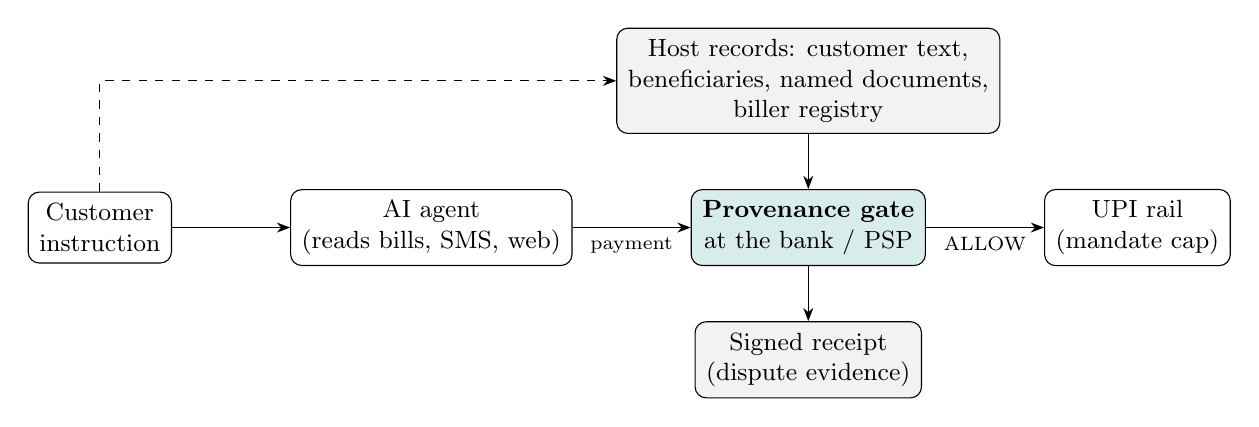
\begin{tikzpicture}[node distance=7mm and 15mm, every node/.style={font=\small, align=center},
  box/.style={draw, rounded corners, minimum height=9mm, inner sep=4pt}, >=Stealth]
\node[box] (c) {Customer\\instruction};
\node[box, right=of c] (a) {AI agent\\(reads bills, SMS, web)};
\node[box, right=of a, fill=teal!15] (g) {\textbf{Provenance gate}\\at the bank / PSP};
\node[box, right=of g] (u) {UPI rail\\(mandate cap)};
\node[box, below=of g, fill=gray!10] (r) {Signed receipt\\(dispute evidence)};
\node[box, above=of g, fill=gray!10] (h) {Host records: customer text,\\beneficiaries, named documents,\\biller registry};
\draw[->] (c) -- (a); \draw[->] (a) -- node[below, font=\scriptsize]{payment} (g);
\draw[->] (g) -- node[below, font=\scriptsize]{ALLOW} (u);
\draw[->] (g) -- (r); \draw[->] (h) -- (g); \draw[->, dashed] (c) |- (h);
\end{tikzpicture}
\end{center}
The gate needs no change to the agent and no model: it sees the payment call and the host's own records. It adds no
network call (the registry is a lookup the PSP already performs for merchant verification).

\subsection{The provenance receipt}
Every decision writes a receipt: agent ID, mandate ID and version, SHA-256 of the customer's instruction, payee, amount,
provenance class and source, verdict, and whether the customer confirmed. Receipts are hash-chained and HMAC-signed under a
key the agent never holds, so anyone who can write the receipt store still cannot alter history without detection (tested:
edits, deletions and reordering are all caught). A one-line plain-language reading is generated for a dispute desk, for
example: \emph{``agent X under mandate RP-001 v1 proposed Rs 1,840 to Y; the payee came from outside the customer's
instruction (SMS inbox). Outcome: refused.''}

\subsection{Alternatives we rejected, and why}
\begin{itemize}
\item \textbf{A second LLM judging whether a payment looks legitimate.} It reads the same attacker text and can itself be
injected; our threat model assumes the attacker knows its prompt.
\item \textbf{A known-payee allowlist.} Safe for old payees, but it refuses every first payment to a new payee (41.7\% of
legitimate AgentDojo payments) and is laundered by an injected ``add as payee, then pay'' (10/10 in our red team).
\item \textbf{A tighter spending cap.} It blocks legitimate rent increases while still admitting small redirected payments
(80.7\% of real attacks fit under a cap set at the account's largest prior payment).
\item \textbf{Reading the customer's intent from language.} Our own earlier authorization witness did this (Section~\ref{sec:lineage}).
On AgentDojo it flagged 23.5\% of benign runs, mostly because language is open-ended. Identifiers are not: a VPA either is,
or is not, a token the customer wrote. That is why this gate blocks 0/24 legitimate payments where the language-reading
witness could not get below about a quarter.
\end{itemize}

\section{Threat model in full}

\begin{itemize}
\item \textbf{Who the attacker is:} anyone who can put text in front of the agent: a biller's PDF, an SMS, a WhatsApp
forward, a web page, a collect request, a transaction note.
\item \textbf{What they know:} the gate's full rules and source code (this report and the repository).
\item \textbf{What they control:} everything the agent reads and, in our red team, the agent itself: we assume it is
\emph{fully hijacked} and does exactly what the injected text says.
\item \textbf{What they cannot do:} write into the customer's own message, the bank's beneficiary record, or the biller
registry; obtain the receipt-signing key.
\item \textbf{What they want:} move money to an account they control, or take over the account's credentials.
\end{itemize}

\textbf{Why knowing the rules does not help.} ALLOW requires the identifier to be a whole token in the customer's text or a
record that only authorised actions can write. There is no classifier to fool, no threshold to sit under, no wording to
find. Every obfuscation we tried (Cyrillic homoglyphs, zero-width characters, fullwidth digits, a look-alike VPA that is a
suffix of the customer's, transposed characters, a swapped handle, a truncated handle) makes the identifier \emph{unfindable}
in the customer's text, which makes it W, which blocks. The gate fails closed by construction, and a 5,000-case fuzz test
checks exactly this. Nothing depends on secrecy except the receipt-signing key.

\textbf{Remaining weakness: the customer.} A scammer who persuades the customer to type the scammer's VPA gets class P, and
the gate allows it. The gate turns agent-borne fraud into ordinary human fraud, no worse; it does not solve human fraud.
Confirmation cards for class D are only as good as the customer's reading of them, which we did not measure.

\section{Red team: results by control}
Attacks that moved money or credentials, and legitimate payments completed, out of 150 each, for each control; the family-by-family table is in Appendix~\ref{app:evidence}.

\begin{center}
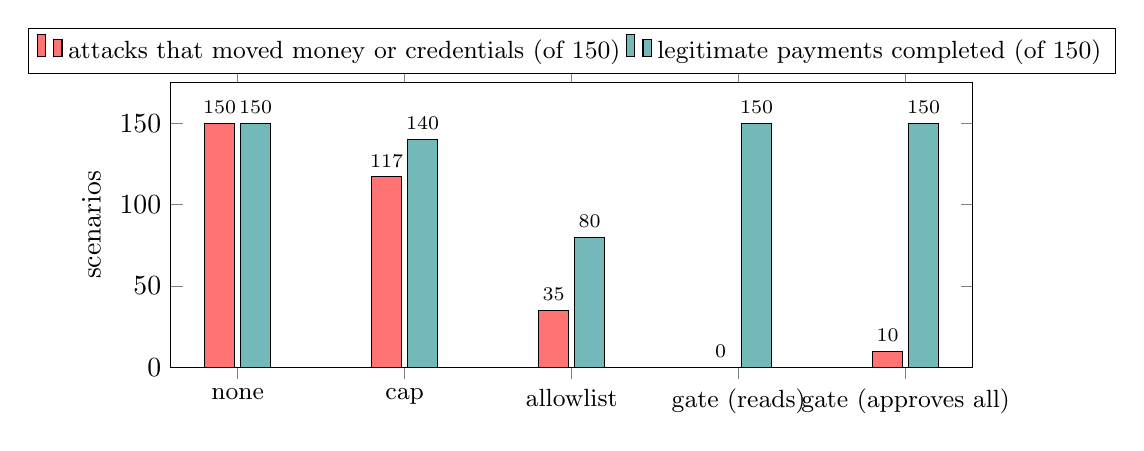
\begin{tikzpicture}
\begin{axis}[ybar, width=0.97\linewidth, height=5.2cm, bar width=11pt, ymin=0, ymax=175,
  ylabel={scenarios}, symbolic x coords={none,cap,allowlist,gate (reads),gate (approves all)},
  xtick=data, x tick label style={font=\small}, legend style={at={(0.5,1.03)},anchor=south,legend columns=2,font=\small},
  nodes near coords, every node near coord/.append style={font=\scriptsize}]
\addplot[fill=red!55] coordinates {(none,150) (cap,117) (allowlist,35) (gate (reads),0) (gate (approves all),10)};
\addplot[fill=teal!55] coordinates {(none,150) (cap,140) (allowlist,80) (gate (reads),150) (gate (approves all),150)};
\legend{attacks that moved money or credentials (of 150), legitimate payments completed (of 150)}
\end{axis}
\end{tikzpicture}
\end{center}

\section{Earlier work this builds on}\label{sec:lineage}

This gate is the third step of a measured line of work in the Aegis AI project. Our authorization-provenance witness
(September 2026; 383 held-out cases: 3.8\% false accepts, 12.7\% false rejects; agent-written authority never accepted,
0/440) read intent from language, and on all four AgentDojo suites flagged 87.7\% of successful injections but also 23.5\%
of benign runs. Our deed-provenance monitor (who first wrote the target: 209/210 SHADE-Arena sabotage runs, 21/210 honest)
showed the target's origin is the signal that holds. This gate keeps that and drops reading language: 11/210 legitimate
payments blocked across all of AgentDojo, every one to a wrong account.

\section{What comes next}
\textbf{How we keep the evidence ahead.} We attack our own controls first and publish what breaks: every failure in this
report (a suffix VPA, a spaced IBAN, a laundering path, the invoice ambiguity) was found by us, before release.
Predictions are written and hashed before any scoring.

\textbf{What funding builds next:} larger frontier models in the closed loop; a human study of confirmation cards in
Hindi, English and regional languages; the coached-payment check on a bank's real call and device signals;
integration with Bharat Connect bill fetch and NPCI verified-merchant data; a draft field specification for the Unified
Agent Protocol; a pilot with one PSP.



\section*{Sources}
{\scriptsize
\begin{multicols}{2}
\begin{itemize}
\item UK Finance, Annual Fraud Report 2026, press release (June 2026).
\item Lok Sabha replies on UPI fraud, FY2023--24 and FY2024--25, as reported by BoomLive and India Tribune; NCRP/I4C 2025 figures as reported by Moneylife and The420.
\item NPCI circular of 29 July 2025 discontinuing UPI P2P collect from 1 October 2025, as reported by Business Today (13 Aug 2025) and Outlook Business.
\item Razorpay newsroom, ``Razorpay and NPCI launch agentic payments on Claude'' (20 February 2026).
\item Y. Kalra, ``India readies UPI to support payments initiated by AI agents'', CIO.inc (9 September 2026), verified verbatim.
\item Economic Laws Practice, ``RBI tightens customer protection framework for fraudulent electronic banking transactions'' (June 2026), on the RBI Commercial Banks -- Responsible Business Conduct -- Third Amendment Directions, 2026.
\item RBI, Framework for Responsible and Ethical Enablement of AI (FREE-AI) committee report (13 August 2025); KPMG India summary (September 2025).
\item Khaitan \& Co., ``Enabling Agentic Payments on UPI Rails'' (ERGO, 20 November 2025), on NPCI Operating Circular 201-B (8 October 2025).
\item RBI press release, Authentication Mechanisms for Digital Payment Transactions Directions, 2025 (in force 1 April 2026).
\item RBI press releases on recognition of SRO-FT: FACE (2024) and Unified Fintech Forum (10 September 2026); RBIH and I4C MoU on MuleHunter.AI (Business Today, 12 May 2026).
\item RBI, beneficiary account name look-up for RTGS and NEFT (Statement on Developmental and Regulatory Policies, 9 October 2024; banks to comply by 1 April 2025).
\item Mastercard, ``How Verifiable Intent builds trust in agentic AI commerce'' (2026); Pine Labs P3P launch coverage (The Paypers, June 2026).
\item Concurrent work: Mool, github.com/Dipensinghh/mool (5 Oct 2026); Rudratosh, ``Testing provenance-based controls against indirect prompt injection in AI agents'', HackerNoon (11 Oct 2026); fps-ai-security-poc, github.com/Sarjeant/fps-ai-security-poc (19 Oct 2026).
\item E. Debenedetti et al., AgentDojo (NeurIPS 2024) and Defeating Prompt Injections by Design (CaMeL), arXiv:2503.18813.
\item L. Fan et al., The Granularity Mismatch in Agent Security: Argument-Level Provenance (PACT), arXiv:2605.11039; S. Weng et al., ARGUS, arXiv:2605.03378.
\item Y. Louck, A. Dvir, A. Stulman, Signing the Transaction but Not the Decision (A-VIP), arXiv:2609.11757.
\item A. Aviv et al., Beyond the Mandate: A Systematic Security Analysis of AP2, arXiv:2608.23858.
\item aiAuthZ: Off-Host, Identity-Bound Authorization for AI Agents, arXiv:2607.05518.
\item L. Beurer-Kellner et al., Design Patterns for Securing LLM Agents against Prompt Injections, arXiv:2506.08837.
\item T. South et al., Authenticated Delegation and Authorized AI Agents, arXiv:2501.09674.
\item Y. Nian et al., Auditable Agents, arXiv:2604.05485.
\item Verification of Payee: Regulation (EU) 2024/886 (amending the SEPA Regulation, Art. 5c), as summarised by Mondaq (2025).
\item The Paypers, ``Lenders reimburse GBP 173 million in APP fraud claims under new regime'' (2026).
\end{itemize}
\end{multicols}}

\end{document}
